%%%%%%%%%%%%%%%%%%%%%%%%%%%%%%%%%%%%%%%%%%%%%%%%%%%%%%%%%%%%%%%%%%%%%%%%%%%%%%%%
%2345678901234567890123456789012345678901234567890123456789012345678901234567890
%        1         2         3         4         5         6         7         8

\documentclass[letterpaper, 10 pt, conference]{ieeeconf}  % Comment this line out if you need a4paper

%\documentclass[a4paper, 10pt, conference]{ieeeconf}      % Use this line for a4 paper

\IEEEoverridecommandlockouts                              % This command is only needed if 
                                                          % you want to use the \thanks command

\overrideIEEEmargins                                      % Needed to meet printer requirements.

% See the \addtolength command later in the file to balance the column lengths
% on the last page of the document

% The following packages can be found on http:\\www.ctan.org
%\usepackage{graphics} % for pdf, bitmapped graphics files
%\usepackage{epsfig} % for postscript graphics files
%\usepackage{mathptmx} % assumes new font selection scheme installed
%\usepackage{times} % assumes new font selection scheme installed
%\usepackage{amsmath} % assumes amsmath package installed
%\usepackage{amssymb}  % assumes amsmath package installed

\usepackage[pdftex]{graphicx}

%\graphicspath{}

\title{\LARGE \bf
Influence of child-robot spacial arrangement in a learning by teaching task}


\author{A1$^{1}$ and A2$^{2}$% <-this % stops a space
\thanks{}% <-this % stops a space
\thanks{$^{1}$A1 is with Faculty of A1,
        University of A1, country
        {\tt\small A1 email}}%
\thanks{$^{2}$A2 is with Faculty of A2,
        University of A2, country
        {\tt\small A2 email}}%
}


\begin{document}



\maketitle
\thispagestyle{empty}
\pagestyle{empty}


%%%%%%%%%%%%%%%%%%%%%%%%%%%%%%%%%%%%%%%%%%%%%%%%%%%%%%%%%%%%%%%%%%%%%%%%%%%%%%%%
\begin{abstract}
In this paper we present a study in which we test the influence of child-robot spatial arrangement on child's focus of attention, child's perception of robot's performance in the CoWriter learning by teaching activity.
In this activity the child teaches a Nao robot how to handwrite. 
In our study, we explore two spatial condition from Kendon's F formation, the side-by-side and the face-t-face formations. 

We have 2 conditions following Kendon's F formation: 
\begin{itemize}
\item side by side
\item face to face
%\item in L shape
\end{itemize}



\end{abstract}


%%%%%%%%%%%%%%%%%%%%%%%%%%%%%%%%%%%%%%%%%%%%%%%%%%%%%%%%%%%%%%%%%%%%%%%%%%%%%%%%
\section{INTRODUCTION}
Interaction settings are crucial for 

Robots to enhance childhood education


The Co-Writer projects aims to help children with difficulties in handwriting \cite{hood2015when}. 
It is based on the idea of learning by teaching. 
By teaching a Nao robot how to write, children learn and improve their handwriting. 
The activity also plays with the protégé effect that make children more motivated in practising for the robot than for themselves. 

Previous studies in the Co-Writer project helped us to develop a system that generates handwriting for the robot based on demonstrations from the child\cite{hood2015when}. 
Case studies presented in \cite{jacq2016building} showed that children were able to stay engaged in long term interaction with repeated session within the Co-Writer activity in real pedagogical/therapeutic contexts. 
These works proved to have a positive effect on extrinsic motivation of children when practising their handwriting thanks to the protégé effect. 

\cite{Matsuzoe2012} had a similar approach than learning by teaching with their Care Receiving Robot that was being taken cared off and taugh by a child with physical interaction. 



Proxemics : explain how spatial arrangement could influence the interaction

Role attribution

Kendon F Formation in HRI: explain how spatial arrangement had influences in the past

Spatial arrangement is also a social signal that tells about the relationship between the persons.



\cite{huttenrauch2006investigating}

We propose to study the impact of spatial arrangement on engagement of children a handwriting task


\section{RELATED WORKS}


Perspective taking: speaker with partners tend yo use more egocentric perspective rather than solo speakers \cite{Schober} 

Handwriting linked to spatial-sequential ability of the child. 
This is also linked to perspective taking ability of the child. 

The 3 spatial perspective taking rules state that :
\begin{enumerate}
\item any object will present the same visual appearance to the self and to another person if the two observer view from the same point of view.
\item An object with different sides will be seen different if the viewers are form different side views
\item An object homogeneous in all sides will be the same from different view. 
\end{enumerate}




\cite{Newcombe1992} shows that children around the age of 5 are able to complete perspective taking tasks and to imagine what others point of you might look like.




\section{APPROACH}
In this study, each child saw interacted with the robot in the two conditions in a random order. 


within subjects Repeated measures 


Hypothesis
\begin{itemize}
\item Child feels more in a teacher student relationship when facing the robot
\item child feels more in a peer to peer when the robot is in L or side by side 
\item how does it influence the engagement -> with-me-ness
\item  does the child looks more at the experimenter when the robot is badly behaving
\item how does the child rates the robots performances according to  the arrangement
\end{itemize}


\section{METHOD}
25

Number of child
Expe settings
Condition within subject but with 
\begin{figure}[t!]
    \centering
        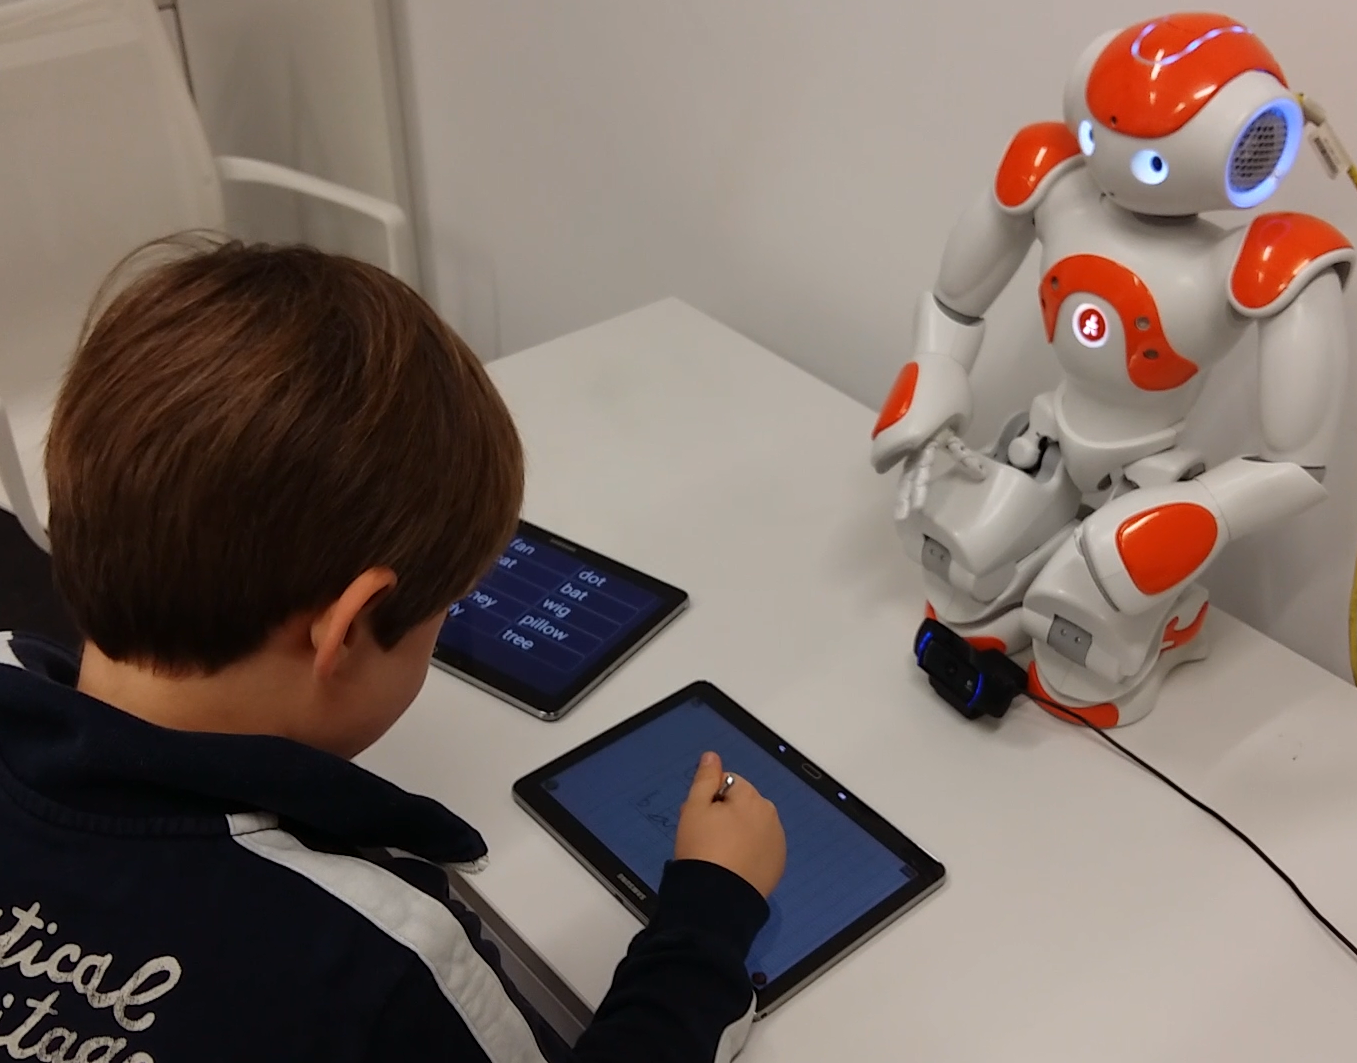
\includegraphics[height=1.2in]{./figures/f2f_photo.png}
        \caption{Face to face spatial formation}
   ~
        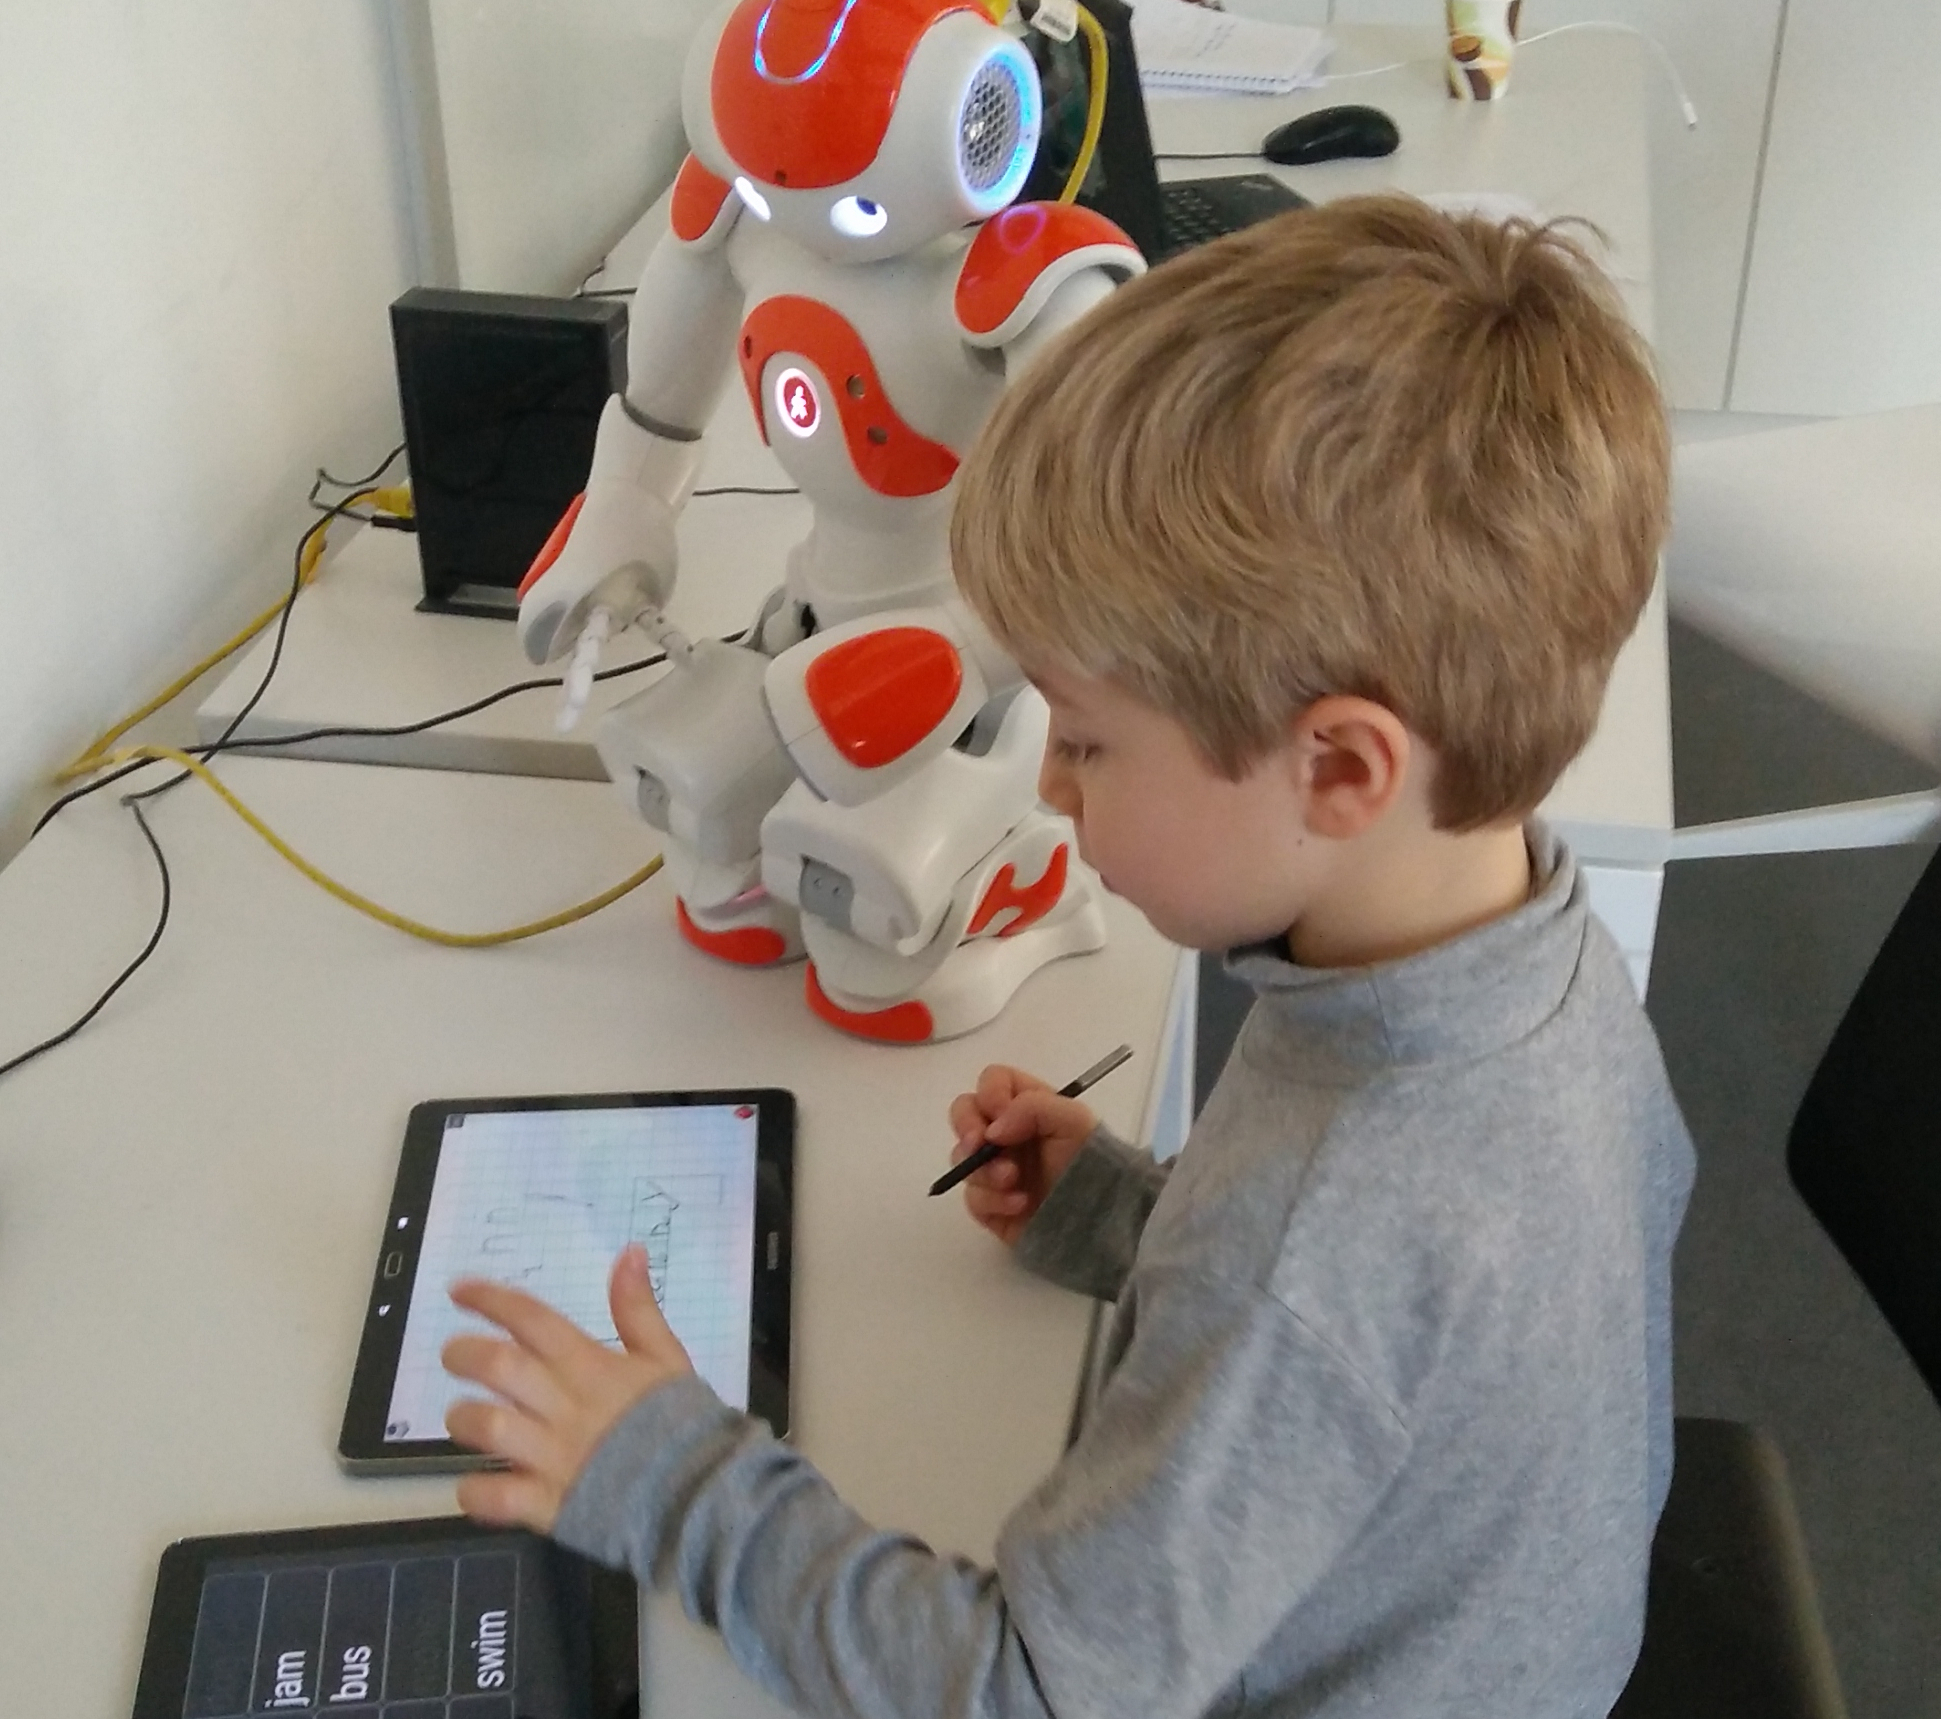
\includegraphics[height=1.2in]{./figures/s2s_photo2.jpg}
        \caption{Side by Side spatial formation}
\end{figure}


\subsection{Reward Mechanism}
The table interface on which the child and the robot practice their handwriting contains also two buttons that allow the child to give positive (green thumb-up) or negative (red thumb-down) feedback to the robot's handwriting.

We noticed that children were expecting the robot to react. 
Now that the usage of these buttons have been proven, we will consider for future experiment to allow the robot to react. 
For instance, if the child gives a positive feedback when the robot is actually improving, the robot should display a positive emotion.
If he is given a positive feedback but doesn’t not actually make any progress, he might express doubt to force the child to be more exigent. 


\subsection{With-me-ness}
The with-me-ness measure applied in HRI in \cite{lemaignan2016realtime}, helps to set specific targets during each state of the interaction and to determine rather the user is looking at one of these targets or not. 
The algorithm is based on the d-lib library that helps to estimate the head pose of the user using a video from webcam device for instance.

This measure allow us to see if the child is engage in the interaction and is looking at the tablet or the robot's head when he/she should.

For this experiment, the targets where: "the observer"(a teacher or a teacher assistant), "the selection tablet"(the tablet used to pick a word), 

Present it as a measure of synchrony, 

Get time when robot looking where and see if similar pattern with child

\subsection{Performances}


\section{RESULTS}

\subsection{Reward Mechanism}
 


\subsection{With-me-ness}


\subsection{Performances}


\section{CONCLUSIONS}



\addtolength{\textheight}{-12cm}   % This command serves to balance the column lengths
                                  % on the last page of the document manually. It shortens
                                  % the textheight of the last page by a suitable amount.
                                  % This command does not take effect until the next page
                                  % so it should come on the page before the last. Make
                                  % sure that you do not shorten the textheight too much.

%%%%%%%%%%%%%%%%%%%%%%%%%%%%%%%%%%%%%%%%%%%%%%%%%%%%%%%%%%%%%%%%%%%%%%%%%%%%%%%%



%%%%%%%%%%%%%%%%%%%%%%%%%%%%%%%%%%%%%%%%%%%%%%%%%%%%%%%%%%%%%%%%%%%%%%%%%%%%%%%%



%%%%%%%%%%%%%%%%%%%%%%%%%%%%%%%%%%%%%%%%%%%%%%%%%%%%%%%%%%%%%%%%%%%%%%%%%%%%%%%%

\section*{ACKNOWLEDGMENT}
This research was partially supported by the Funda\c{c}\~{a}o para a Ci\^{e}ncia
e a Tecnologia (FCT) with reference UID/CEC/ 50021/2013, and by the Swiss
National Science Foundation through the National Centre of Competence in
Research Robotics.



%%%%%%%%%%%%%%%%%%%%%%%%%%%%%%%%%%%%%%%%%%%%%%%%%%%%%%%%%%%%%%%%%%%%%%%%%%%%%%%%




\bibliographystyle{abbrv}
\bibliography{fformation_cowriter}


\end{document}
